\documentclass{beamer}


\usepackage[T1]{fontenc}
\usepackage{textcomp} 

\usepackage{futura}
\usetheme{Antibes}
\usecolortheme{beetle}

\title{Prediction of reliability and method effects in surveys from characteristics of the questions}
\author{Daniel Oberski}
\institute
{
  \inst{}%
  Faculty of Social and Behavioural Sciences\\
  Tilburg University
  \and
  \inst{}%
  Survey Research Centre of Catalunya\\
  ESADE, Barcelona\\
  Universitat Ramon Llull\vspace{-1.2cm}
}
\date{}

\begin{document}

\begin{frame}
	\titlepage
	\begin{center}
	 \includegraphics[width=4.5cm]{i/uvttransparent.png}\hspace{.2cm}
	 
\includegraphics[width=2.8cm]{i/esade.png}	
  \end{center}	
\end{frame}

\section*{Outline}

\begin{frame}
\frametitle{Overview}
	\tableofcontents
\end{frame}

\section{Multitrait-multimethod experiments}

\begin{frame}
	\frametitle{An example experiment}
\end{frame}

\subsection{Designs}

\begin{frame}	
	\frametitle{An oversimplified design}
\end{frame}	
\begin{frame}	
	\frametitle{a full 3 trait 3 method design}
\end{frame}	
\begin{frame}	
	\frametitle{a panel design}
\end{frame}	
\begin{frame}	
	\frametitle{a split ballot design}
\end{frame}	

\subsection{Models}

\begin{frame}	
	\frametitle{c-u}
\end{frame}	
\begin{frame}	
	\frametitle{direct product}
\end{frame}	
\begin{frame}	
	\frametitle{MTM-1}
\end{frame}	
\begin{frame}	
	\frametitle{true score uncorrelated methods}
\end{frame}	

\section{What has been done already}

\subsection{The international research project 1984--1996}

\begin{frame}
 \frametitle{The international research project 1984--1996\\and the `old' Survey Quality Predictor}
\end{frame}

\if 1=2
\begin{frame}
%\frametitle{The international research project 1984--1996}
\begin{small}
	\begin{columns}[T]	
		\begin{column}{2.5cm}
			\includegraphics[width=2.2cm]{i/andrews.jpg}\\
			Frank M. Andrews\\	\vspace{.2cm}
			
			\vspace{1cm}
			Richard K\"{o}ltringer			
		
		\end{column}		
		\begin{column}{4cm}
			\includegraphics[width=3.916cm]{i/veldandsaris.jpg}\\
					William	van der Veld \& Willem Saris\\					
			
			
		\end{column}		
		\begin{column}{2.5cm}		
		\includegraphics[width=2.2cm]{i/scherpenzeel.jpg}\\
			Annette Scherpenzeel\\ \vspace{.2cm}
						
		\includegraphics[width=2.2cm]{i/gallhofer.jpg}\\
		 Irmtraud Gallhofer		
		\end{column}		
	\end{columns}
	\end{small}
\end{frame}
\fi

\begin{frame}
\begin{itemize}
	\item Coding scheme, characteristics coded
	\item Question characteristics
	\item Experiment characteristics
\end{itemize}

\end{frame}

\begin{frame}
\frametitle{Countries in the international survey project 1984--1996\\that have been included in SQP}
	\begin{columns}[T]	
		\begin{column}{8cm}
			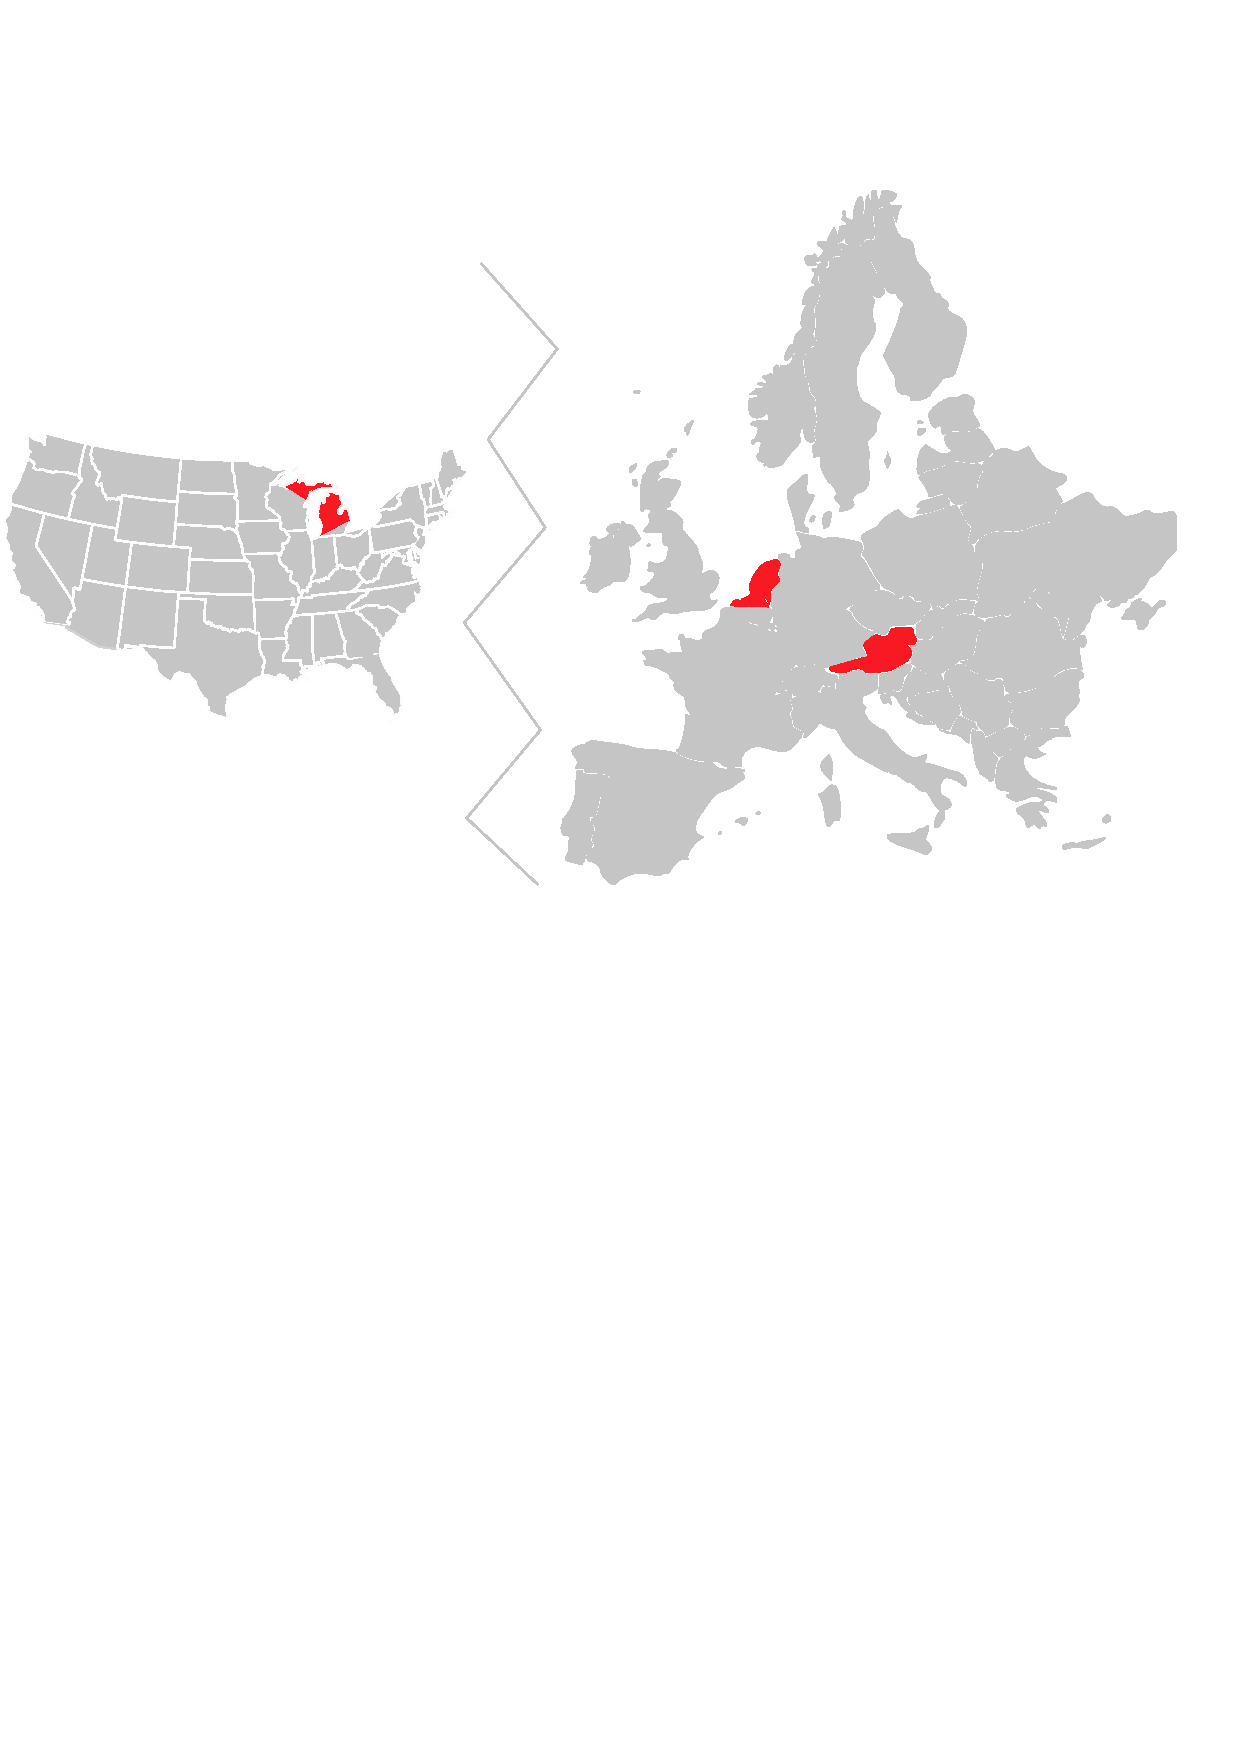
\includegraphics[width=\textwidth]{i/andrews-etal.pdf}
		\end{column}
		\begin{column}{3.2cm}
		\begin{small}
		\begin{enumerate}
			\item Austria 
			\item Belgium: Flanders
			\item Netherlands
			\item United States: Michigan		
		\end{enumerate}
		\end{small}
		\end{column}
	\end{columns}
\end{frame}

\begin{frame}
 results table and standard errors
\end{frame}

\subsection{Design of experiments for the European Social Survey}

\begin{frame}
\begin{itemize}
	\item Three rounds, 4th coming up
	\item Six experiment in each round
	\item Participating countries for each round (maps)
\end{itemize}
\end{frame}

\begin{frame}

\frametitle{Countries in round 1 of the ESS -- 2002}

	\begin{columns}[T]	
		\begin{column}{5.5cm}
			\includegraphics[width=\textwidth]{i/round1.pdf}
		\end{column}
		\begin{column}{4.5cm}
			\begin{columns}	
				\begin{column}{2.2cm}
					\begin{scriptsize}\begin{enumerate}
						\item Austria
						\item Belgium	
						\item Czech Republic 
						\item Denmark 	
						\item Finland 	
						\item France 	
						\item Germany 	
						\item Greece
						\item Hungary 
						\item Ireland 
						\item Israel 	
						\item Italy 										
					\end{enumerate}\end{scriptsize}
				\end{column}
				\begin{column}{2.5cm}
					\begin{scriptsize}\begin{enumerate}			
						\item[13.] Luxembourg			
						\item[14.] Netherlands
						\item[15.] Norway
						\item[16.] Poland
						\item[17.] Portugal
						\item[18.] Slovenia
						\item[19.] Spain
						\item[20.] Sweden
						\item[21.] Switzerland
						\item[22.] United Kingdom
					\end{enumerate}\end{scriptsize}
				\end{column}
			\end{columns}
		\end{column}
	\end{columns}
\end{frame} % to enforce entries in the table of contents

\begin{frame}

\frametitle{Countries in round 2 of the ESS -- 2004}

	\begin{columns}[T]	
		\begin{column}{6.5cm}
			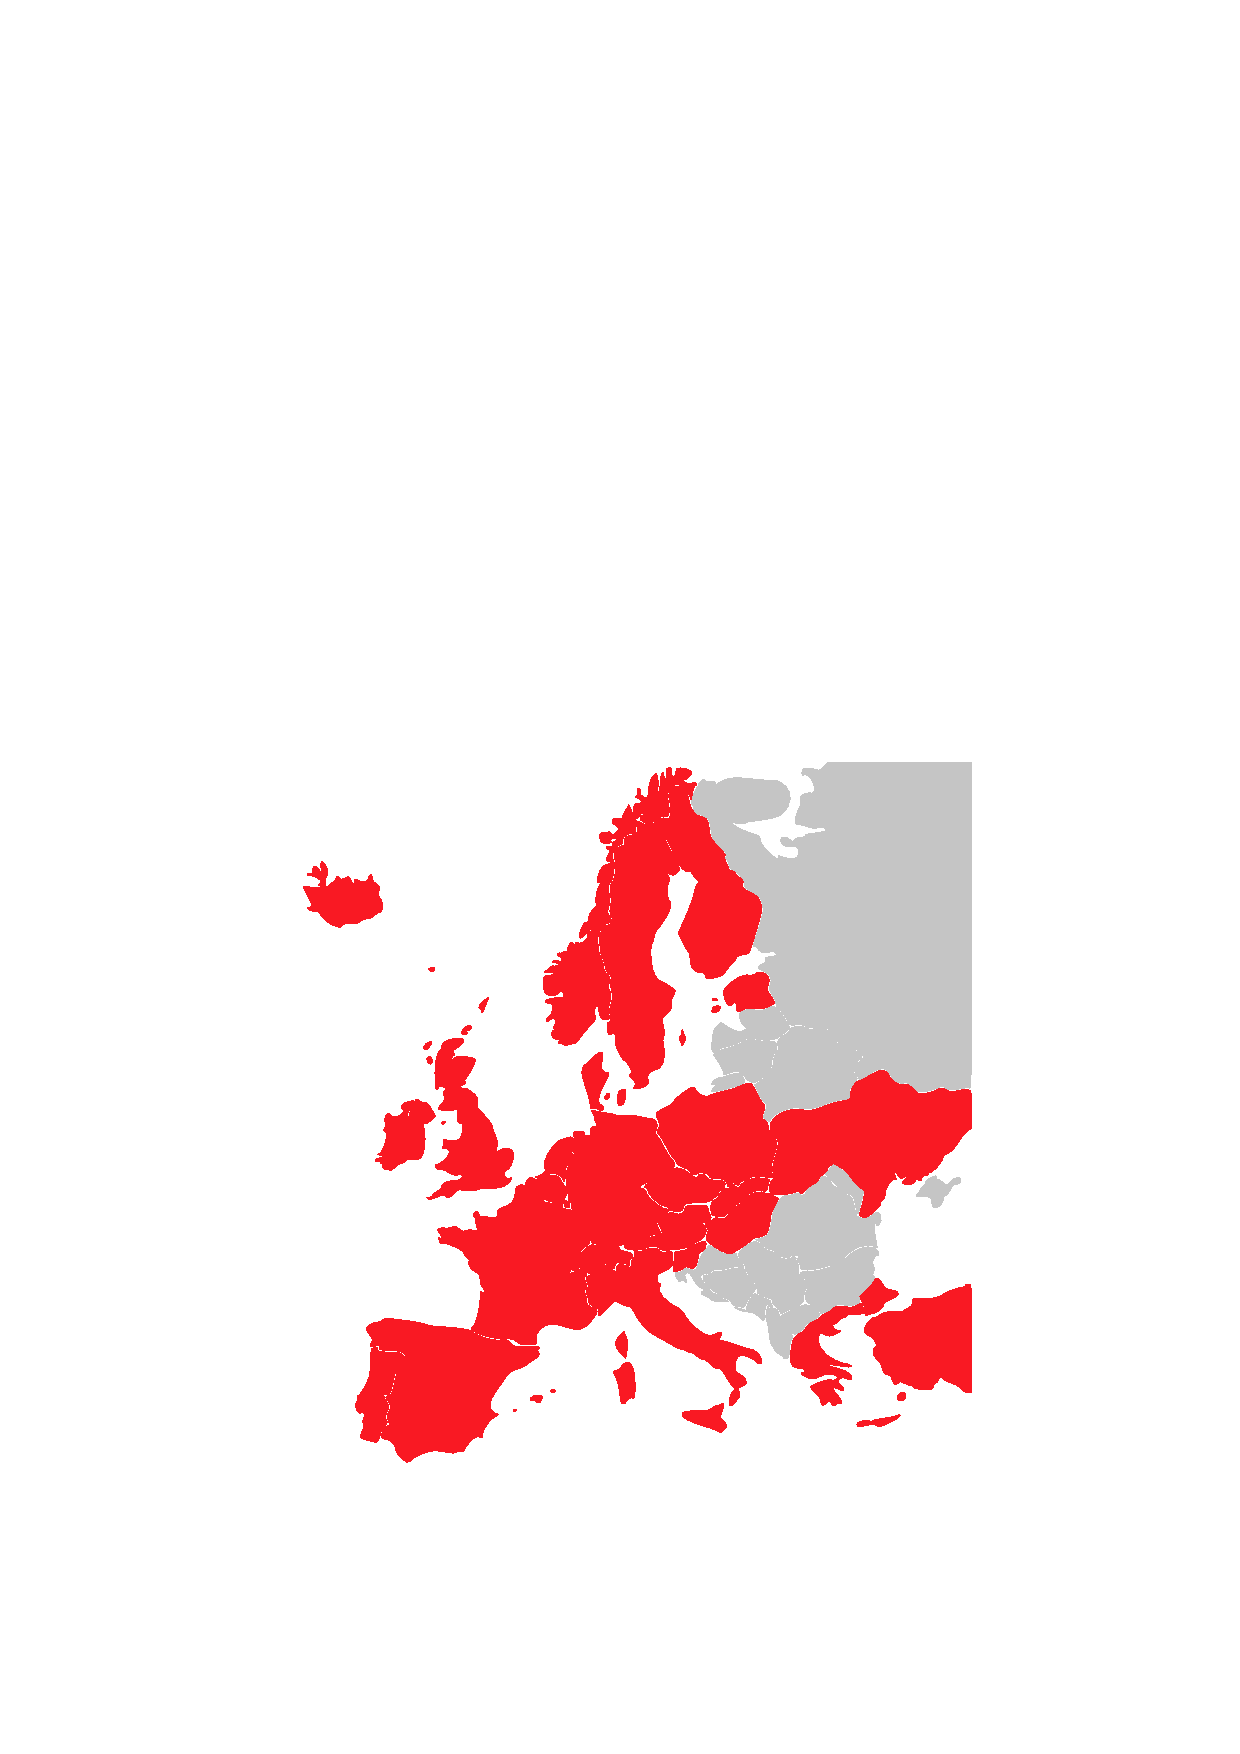
\includegraphics[width=\textwidth]{i/round2.pdf}
		\end{column}
		\begin{column}{4.5cm}
			\begin{columns}	
				\begin{column}{2cm}
					\begin{scriptsize}\begin{enumerate}
            \item Austria 	        
						\item Belgium 	        
						\item Czech Republic 	
						\item Denmark 	        
						\item Estonia 	        
						\item Finland 	        
						\item France 	        
						\item Germany 	        
						\item Greece 	        
						\item Hungary 	        
						\item Iceland 	        
						\item Ireland 	        		
            \item Italy 	
        \end{enumerate}\end{scriptsize}
				\end{column}
				\begin{column}{2.5cm}
					\begin{scriptsize}\begin{enumerate}			
						\item[14.] Luxembourg 	
						\item[15.] Netherlands 	
						\item[16.] Norway 	
						\item[17.] Poland 	
						\item[18.] Portugal 	
						\item[19.] Slovakia 	
						\item[20.] Slovenia 	
						\item[21.] Spain 	
						\item[22.] Sweden 	
						\item[23.] Switzerland 	
						\item[24.] Turkey 	
						\item[25.] Ukraine 	
						\item[26.] United Kingdom 						
\end{enumerate}\end{scriptsize}
				\end{column}
			\end{columns}
		\end{column}
	\end{columns}
\end{frame}

\begin{frame}

\frametitle{Countries in round 3 of the ESS -- 2006}

	\begin{columns}[T]	
		\begin{column}{6.5cm}
			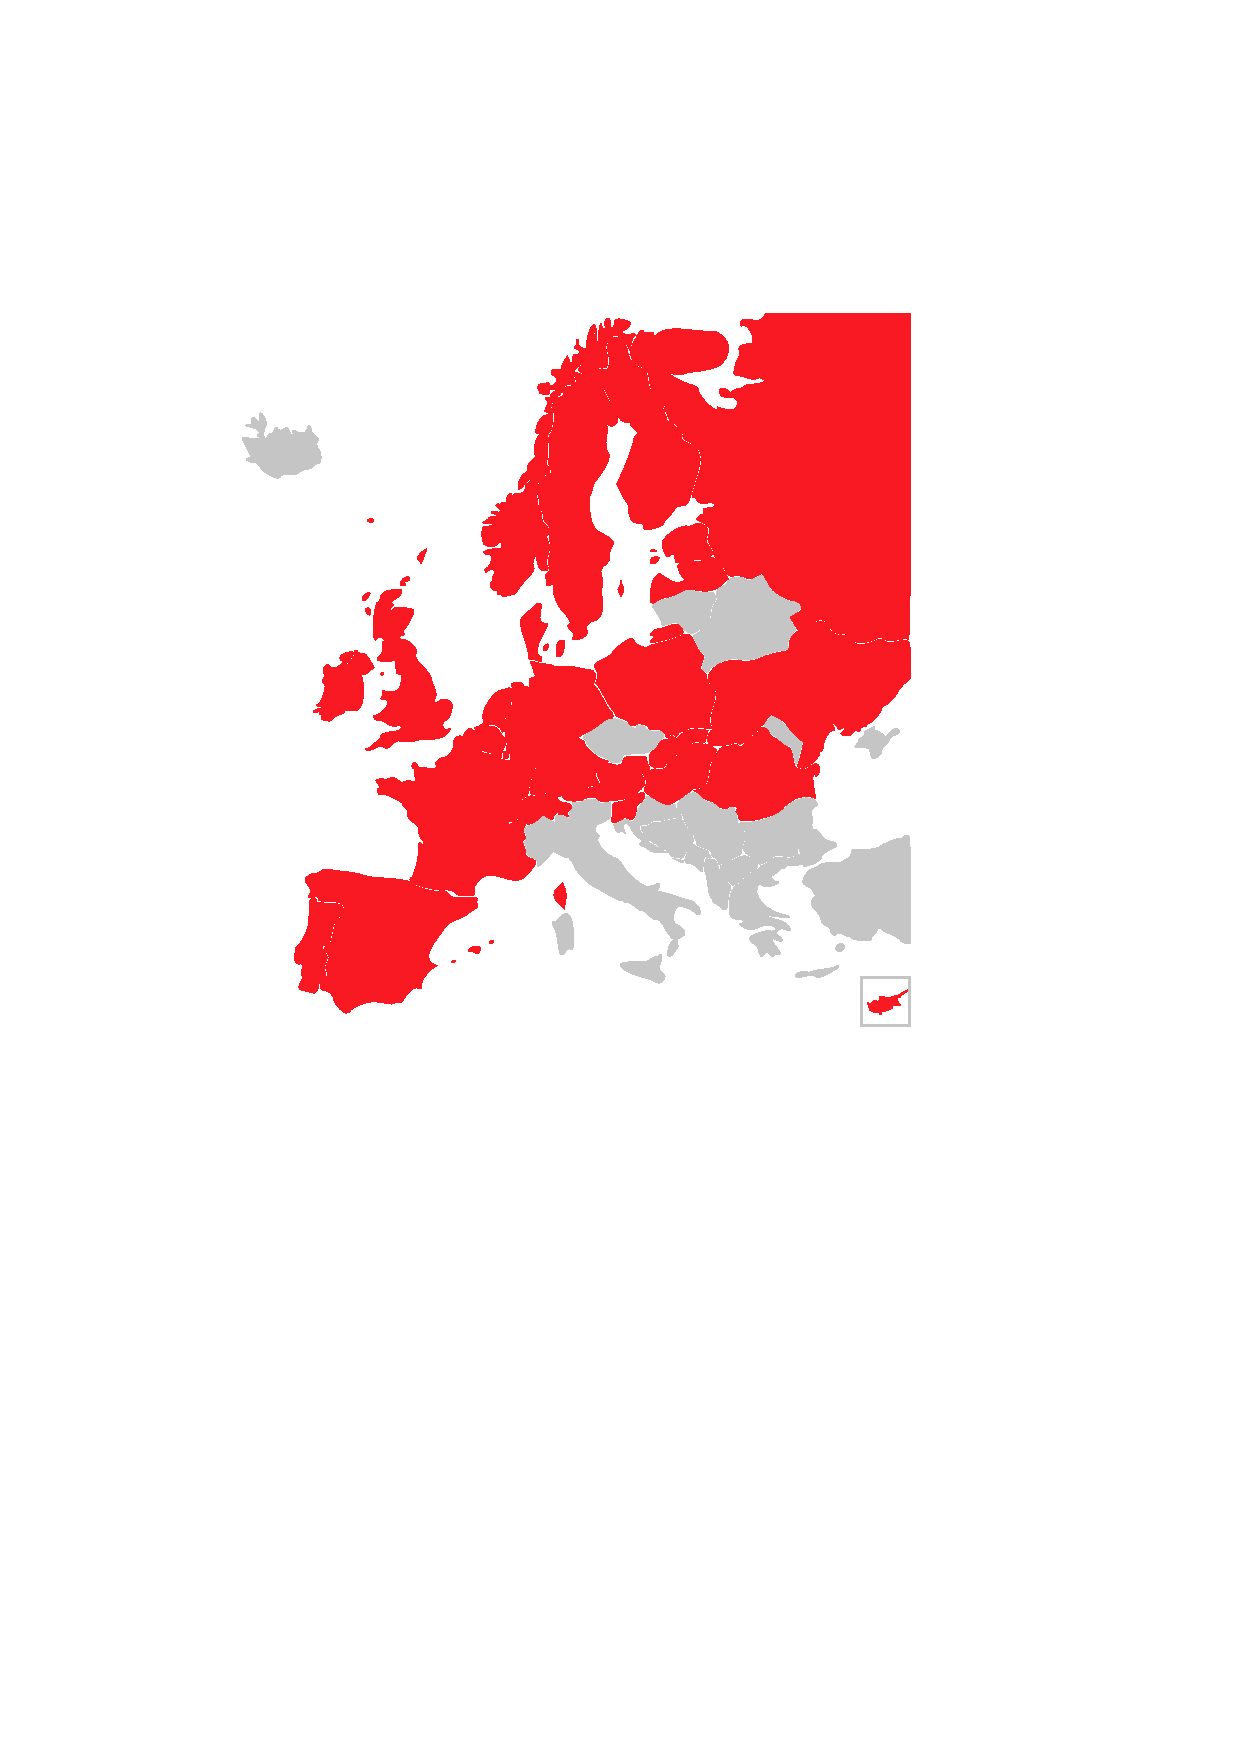
\includegraphics[width=\textwidth]{i/round3.pdf}
		\end{column}
		\begin{column}{4.5cm}
			\begin{columns}	
				\begin{column}{2cm}
					\begin{scriptsize}\begin{enumerate}
						\item Austria
						\item Belgium 	
						\item Bulgaria 	
						\item Cyprus 	
						\item Denmark 	
						\item Estonia 	
						\item Finland 	
						\item France 	
						\item Germany 	
						\item Hungary 	
						\item Ireland
						\item Latvia													
					\end{enumerate}\end{scriptsize}
				\end{column}
				\begin{column}{2.5cm}
					\begin{scriptsize}\begin{enumerate}		
						\item[13.] Netherlands			
						\item[14.] Norway 	
						\item[15.] Poland 	
						\item[16.] Portugal 	
						\item[17.] Romania 	
						\item[18.] Russian Federation 	
						\item[19.] Slovakia 	
						\item[20.] Slovenia 	
						\item[21.] Spain 	
						\item[22.] Sweden 	
						\item[23.] Switzerland 	
						\item[24.] Ukraine
						\item[25.] United Kingdom 
					\end{enumerate}\end{scriptsize}
				\end{column}
			\end{columns}
		\end{column}
	\end{columns}
\end{frame}
% topics

\subsection{Survey Quality Predictor: SQP for Windows}
% show workings / demonstration?

\section{Construction of a question database}

\subsection{Coding of the new questions}
\subsection{Storage of questionnaires}

\section{Meta-analysis of mtmm experiments}

\subsection{The model so far}



\begin{frame}	
	\frametitle{Our/other's ideas so far}
\begin{itemize}
	\item Weight by standard errors
	\item Beta regression
	\item Interval prediction
	\item Perhaps easier to make a bayesian model
\end{itemize}

\end{frame}	

\section{New version of SQP}

% web based --> all platforms
% 

\section{Questions for the audience}
% IRT rather than standard factor models?
% mixture/ latent class models?
% model for the meta-analysis?
% any methodological problems with design?


\begin{frame}
\end{frame}

\end{document}
